\documentclass[a4paper, onecolumn, 11pt, longbibliography]{quantumarticle}
\pdfoutput=1

\usepackage{silence}
\WarningFilter{caption}{Unknown document class}

\usepackage[linesnumbered, ruled, vlined]{algorithm2e}
\usepackage{amsmath, amssymb, amsthm, mathrsfs, amsfonts, dsfont}
\usepackage{bbm}
\usepackage{bm}
\usepackage{booktabs}
\usepackage{braket}
\usepackage{calc}
\usepackage[style=base]{caption}
% \usepackage{csvsimple}
\usepackage{enumerate}
\usepackage{enumitem}
% \usepackage{epsfig}
\usepackage{hyperref}
\usepackage[margin=1in]{geometry}
\usepackage[dvipdfmx]{graphicx}
\usepackage{ifthen}
% \usepackage{listings}
\usepackage{lipsum}
\usepackage{makecell}
\usepackage{mathtools}
\usepackage{multirow}
\usepackage{nicematrix}
\usepackage{optidef}
\usepackage{physics}
% \usepackage{qcircuit}
% \usepackage{siunitx}
% \usepackage{stfloats}
\usepackage{subfiles}
\usepackage{subcaption}
\usepackage{thm-restate}
\usepackage{tikz}
% \usepackage[hyphens]{url}
\usepackage{xparse}
% \usepackage[all]{xy}
\usepackage{xparse}
\hypersetup{colorlinks=true,linkcolor=blue,citecolor=blue,urlcolor=blue}

% === Commands ===

\newcommand{\red}[1]{\textcolor{red}{#1}}
\newcommand{\blue}[1]{\textcolor{blue}{#1}}
\newcommand{\cyan}[1]{\textcolor{cyan}{#1}}
\newcommand{\gray}[1]{\textcolor{gray}{#1}}
\newcommand{\green}[1]{\textcolor{green}{#1}}
\newcommand{\brown}[1]{\textcolor{brown}{#1}}
\newcommand{\black}[1]{\textcolor{black}{#1}}
\newcommand{\orange}[1]{\textcolor{orange}{#1}}
\newcommand{\purple}[1]{\textcolor{purple}{#1}}
\newcommand{\yellow}[1]{\textcolor{yellow}{#1}}
\newcommand{\Magenta}[1]{\textcolor{Magenta}{#1}}
\newcommand{\RoyalBlue}[1]{\textcolor{RoyalBlue}{#1}}
\newcommand{\RubineRed}[1]{\textcolor{RubineRed}{#1}}
\newcommand{\ForestGreen}[1]{\textcolor{ForestGreen}{#1}}
\newcommand{\YellowOrange}[1]{\textcolor{YellowOrange}{#1}}
\newcommand{\WildStrawberry}[1]{\textcolor{WildStrawberry}{#1}}
\newcommand{\st}{\text{ s.t. }}
\newcommand{\Rank}[1]{\mathrm{rank}\qty(#1)}
\newcommand{\floor}[1]{\left\lfloor #1 \right\rfloor}
\newcommand{\ceil}[1]{\left\lceil #1 \right\rceil}
% C++ (https://tex.stackexchange.com/questions/4302/prettiest-way-to-typeset-c-cplusplus)
\newcommand{\Cpp}{C\nolinebreak[4]\hspace{-.05em}\raisebox{.4ex}{\relsize{-3}{\textbf{++}}}}
% https://tex.stackexchange.com/questions/28836/typesetting-the-define-equals-symbol
\newcommand{\defeq}{\coloneqq}
\newcommand{\eqdef}{\eqqcolon}
% q binomial coefficient
\newcommand{\qBinom}[2]{\genfrac{[}{]}{0pt}{}{#1}{#2}}

% https://tex.stackexchange.com/questions/564216/newcommand-for-each-letter
\ExplSyntaxOn
\NewDocumentCommand{\definealphabet}{mmmm}{
\int_step_inline:nnn{`#3}{`#4}{
\cs_new_protected:cpx{#1 \char_generate:nn{##1}{11}}{
\exp_not:N #2{\char_generate:nn{##1}{11}}}}}
\ExplSyntaxOff

\definealphabet{bb}{\mathbb}{A}{Z}
\definealphabet{rm}{\mathrm}{A}{Z}
\definealphabet{cal}{\mathcal}{A}{Z}
% \definealphabet{scr}{\mathscr}{A}{Z}
\definealphabet{frak}{\mathfrak}{a}{z}
% \definealphabet{frak}{\mathfrak}{A}{Z}

% === Settings ===

\newtheorem{theorem}{Theorem}
\newtheorem{proposition}{Proposition}
\newtheorem{lemma}{Lemma}
\newtheorem{definition}{Definition}
\newtheorem{corollary}{Corollary}
\newtheorem{remark}{Remark}
\newtheorem{example}{Example}

% https://qiita.com/rityo_masu/items/efd44bc8f9229e014237
\allowdisplaybreaks[4]

\usetikzlibrary{
  calc,
  math,
  matrix,
  patterns,
  backgrounds,
  arrows.meta,
}

% This declares a command \Comment
% The argument will be surrounded by /* ... */
% https://ja.overleaf.com/learn/latex/Algorithms
\SetKwComment{Comment}{/* }{ */}

\DontPrintSemicolon

% \graphicspath{{./fig/}}

\providecommand{\main}{.}
\newboolean{isMain}
\setboolean{isMain}{true}

% --------------------  TITLE  --------------------

\begin{document}
\title{Stabilizer Extent Calculation by Column Generation}

% ------------  AUTHORS AND AFFILIATIONS ----------
\author{Hiroki Hamaguchi}
\email{hamaguchi-hiroki0510@g.ecc.u-tokyo.ac.jp}
\affiliation{Graduate School of Information Science and Technology, University of Tokyo, Tokyo, Japan}

\author{Kou Hamada}
\email{zkouaaa@g.ecc.u-tokyo.ac.jp}
\affiliation{Graduate School of Information Science and Technology, University of Tokyo, Tokyo, Japan}

\author{Nobuyuki Yoshioka}
\email{nyoshioka@ap.t.u-tokyo.ac.jp}
\affiliation{Department of Applied Physics, University of Tokyo, Japan}
\affiliation{\orange{Theoretical Quantum Physics Laboratory, RIKEN Cluster for Pioneering Research (CPR), Wako-shi, Saitama 351-0198, Japan}}
\affiliation{\orange{JST, PRESTO, 4-1-8 Honcho, Kawaguchi, Saitama, 332-0012, Japan}}

% --------------------  ABSTRACT  --------------------

\begin{abstract}
    \orange{todo}
\end{abstract}
\maketitle

\section{Introduction}

\orange{todo}
% 方向性?
% 0. quantum resource measureの重要性
% 1. RoMではstabilizer extentへの拡張が示唆されていた
% 2. その拡張可能性は以下の点で自明ではなかった
%   - 内積計算においてFWHTが使えない
%   - LPよりもSOCPの方が一般に難しいクラスの問題である
% 3. 本研究では、stabilizer extentの計算が
%    実際にはCG法を用いて効率的に行えることを示す
%    また、工夫した内積計算により、
%    定数倍を除いて最適な時間計算量のアルゴリズムを提案する
% 4. 結果として、
%    ランダムケースでは...
%    テンソル積の場合では...

\section{Preliminaries}

We denote the entire set of $n$-qubit
stabilizer states as $\calS_n \defeq \qty{\ket{\phi_\alpha}}$.
The size of $\calS_n$
scales superexponentially as
$\abs{\calS_n} = 2^n \prod_{k=0}^{n-1} (2^{n-k} + 1)= 2^{\order{n^2}}$
\cite[Proposition 1]{PhysRevA.70.052328}.
Suppose $\psi$ is a normalized $n$-qubit state.
The \textit{stabilizer extent} is
introduced in~\cite[Definition 3]{Bravyi2019simulationofquantum}
to quantify the state $\psi$,
and is defined as follows:
\begin{equation}\label{eq:stabilizerExtentPrimalOrig}
    \xi(\psi) \defeq \min_{c\in \bbC^{\abs{\calS_n}}} \left\{ \norm{c}_1^2 \;\middle|\; \psi = \sum_{\alpha=1}^{\abs{\calS_n}} c_\alpha \ket{\phi_\alpha} \right\}.
\end{equation}
This definition can be simplified as
complex $L^1$-norm minimization problem:
\begin{equation}\label{eq:stabilizerExtentPrimal}
    \sqrt{\xi(\psi)} = \min_{x \in \bbC^{\abs{\calS_n}}} \left\{ \sum_{\alpha=1}^{\abs{\calS_n}} x_\alpha \;\middle|\; A_n x = b \right\},
\end{equation}
Here, we define $A_n \in \bbC^{2^n \times \abs{\calS_n}}$ as
$(A_n)_{ij} \defeq \braket{i}{\phi_j}$
and $b \in \bbC^{\abs{\calS_n}}$ as
$b_i \defeq \braket{i}{\psi}$
using the computational basis $\qty{\ket{i}}_{i=0}^{2^n-1}$.
As in \cite{heimendahlStabilizerExtentNot2021},
the problem \eqref{eq:stabilizerExtentPrimal}
is a second order cone program (SOCP).
Thus, its dual problem can be derived
~\cite[Appendix A]{heimendahlStabilizerExtentNot2021}\cite[Section 5.1.6]{boydConvexOptimization2004}.
By defining $\calA_n$ as the set of columns $\{a_j\}$ of $A_n$,
\begin{equation}\label{eq:stabilizerExtentDual}
    \sqrt{\xi(\psi)} = \max_{y \in \bbC^{2^n}} \left\{ \Re(b^\dagger y) \;\middle|\; \abs{a_j^\dagger y} \leq 1
    \text{ for all $a_j \in \calA_n$} \right\}.
\end{equation}
where $\dagger$ denotes the conjugate transpose.
Although the actual objective function in~\eqref{eq:stabilizerExtentDual}
should be multiplied by $-1$,
we flipped the sign for simplicity, which does not affect the solution.

In order to describe our algorithm in later sections,
we denote a function $\text{SolveSOCP}(\calC, b)$
which takes a set of columns $\calC$ and a vector $b$,
and returns the optimal solution $E$ and
dual optimal solution $\bm{y}$ of
the SOCP problem~\eqref{eq:stabilizerExtentDual}.
In actual numerical computation,
this function can be realized by just solving
the corresponding primal problem~\eqref{eq:stabilizerExtentPrimal}.

\section{Scaling up The Exact Stabilizer Extent Calculation}

Although SOCP are solvable in polynomial time with
respect to the matrix size,
due to the superexponential growth of
the matrix size $\abs{\calS_n}$,
using the entire $A_n$ is totally impractical
for $n>5$~\cite{}.
In order to tackle this kind of problem,
we have proposed to utilize the
column generation (CG) method
in~\cite{hamaguchiHandbookEfficientlyQuantifying2023}.
The CG method is a well-known technique
to solve large-scale optimization problems.
Here, we show that similar method actually works
for the stabilizer extent calculation too.

\subsection{CG method}

\begin{algorithm}[tb]
    \KwIn{vector $b$ corresponding to the state $\psi$}
    \KwOut{Exact stabilizer extent $\xi(\psi)$}
    \SetKwFunction{SolveSOCP}{SolveSOCP}
    $\calC \gets \text{Partial set of $\calA_n$}$
    \Comment*[r]{Initialize using top overlaps}
    \While{true}{
        $E, \bm{y} \gets \SolveSOCP(\calC, \bm{b})$\\
        $\calC' \gets \qty{\bm{a} \in \calA_n \mathrel{}\middle|\mathrel{} \abs{\bm{a}^\dagger \bm{y}} > 1}$
        \Comment*[r]{Use of subroutine in Section~\ref{sec:coreSubroutine}}
        \If {$\calC' = \emptyset$} {
            \textbf{break}
        }
        $\calC \gets \calC \cup \calC'$\\
    }
    $\Return$ $E$
    \caption{Exact stabilizer extent calculation by Column Generation}
    \label{alg:CG}
\end{algorithm}

\subsection{Core Subroutine: Calculating Overlap}
\label{sec:coreSubroutine}

As a well-known fact,
the stabilizer states have a simple form as shown in the following proposition.
\begin{proposition}[{
                \cite[Theorem 2]{struchalinExperimentalEstimationQuantum2021b},
                \cite[Section 5]{nestClassicalSimulationQuantum2010},
                \cite[Theorem 5.(ii)]{dehaeneCliffordGroupStabilizer2003}
            }]\label{prop:originalStabilizerStateStandardForm}
    All stabilizer states can be written in the following form:
    \begin{equation}\label{eq:stabilizerStateStandardForm}
        \begin{dcases}
            \ket{\phi} \defeq \ket{t}                                                                       & \text{if $k=0$} \\
            \ket{\phi} \defeq \frac{1}{2^{k/2}} \sum_{x=0}^{2^k-1}(-1)^{x^\top Q x} i^{c^\top x}\ket{R x+t} & \text{if $k>0$}
        \end{dcases}
    \end{equation}
    where $Q \in \bbF_2^{k \times k}$, $c \in \bbF_2^k$, $R \in \bbF_2^{k \times (n-k)}$, $t \in \bbF_2^{n-k}$
    and $\Rank{R} = k$.
    Also, any state that can be written in this form is a stabilizer state.
\end{proposition}

\begin{theorem}{Complexity of computing all stabilizer overlaps}
    \label{thm:complexityStabilizerOverlap}
    Computation of $A_n^\dagger y$
    can be done in time complexity of
    $\order{n\abs{S_n}}$ and
    space complexity of $\order{2^n}$.
\end{theorem}

\subsection{For the case $\ket{\psi}$ is Real}
\label{sec:restrictedRealProblem}

\begin{figure}[htbp]
    \centering
    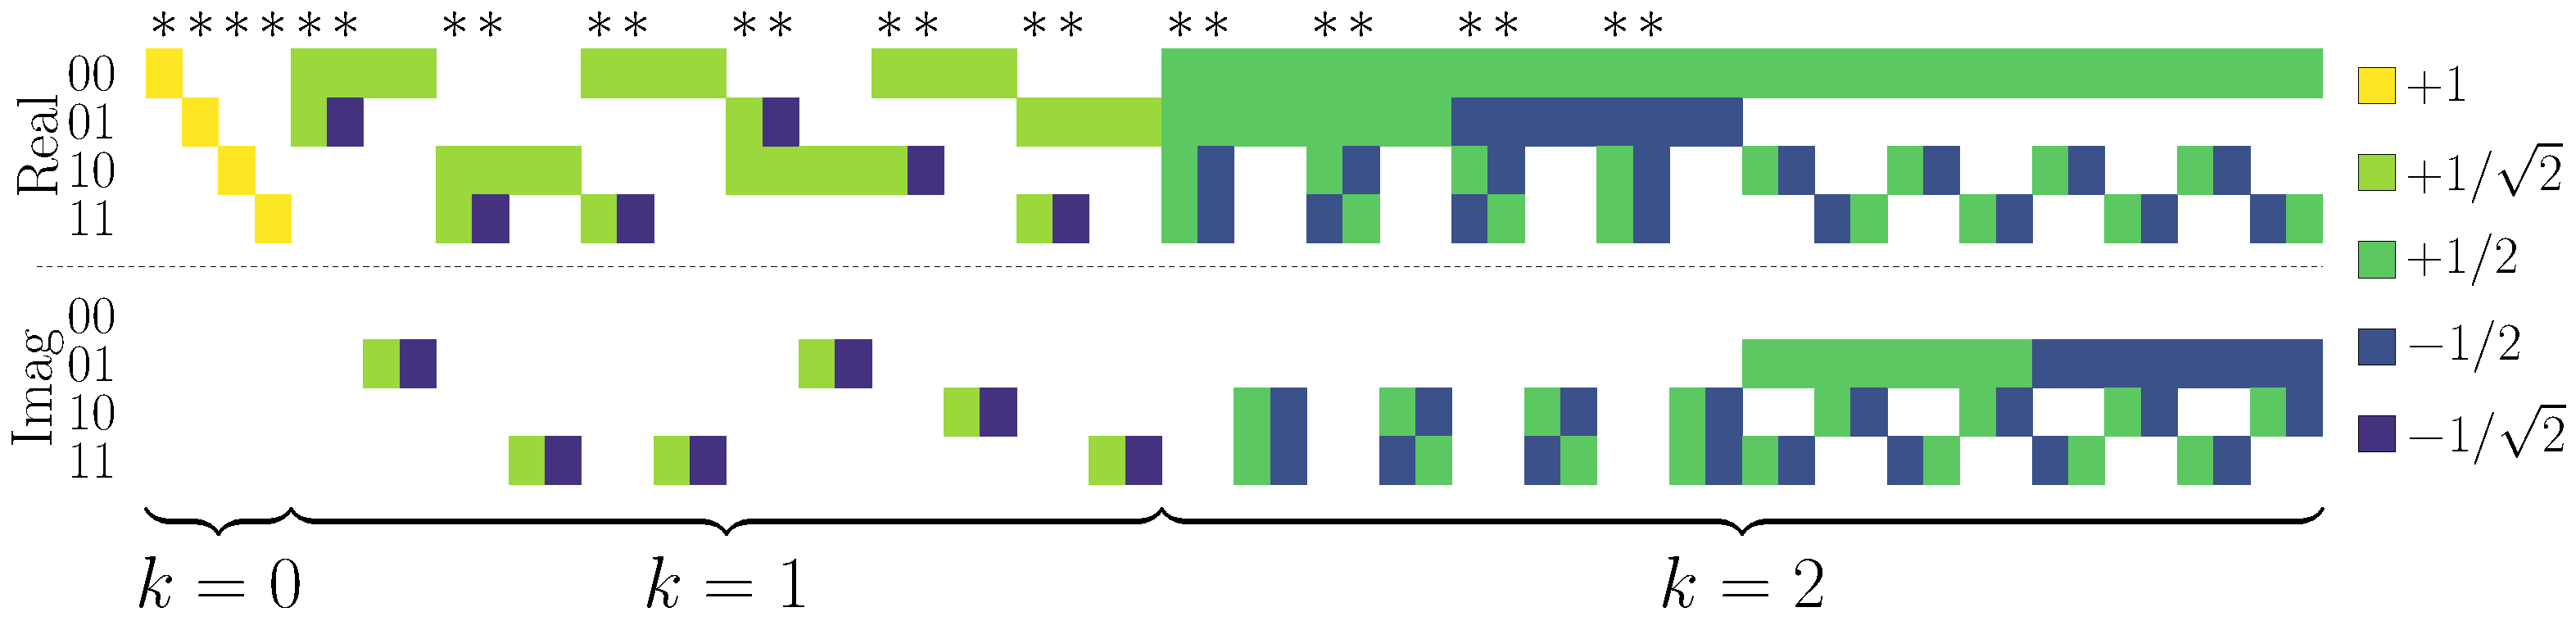
\includegraphics[width=\columnwidth]{imgs/Amat.pdf}
    \caption{
        Visualization of the matrix $A_n$ with $n=2$.
        The upper half corresponds to the real part,
        and the lower half corresponds to the imaginary part.
        The $j$-th column of this represents
        the column $a_j$ and its state $\ket{\phi_j}$.
        The $k$ below the matrix
        corresponds to
        the standard form \eqref{eq:stabilizerStateStandardForm}.
        By restricting the matrix $A_n$
        to the starred columns
        which are real vectors,
        we can obtain the matrix $A_n'$.
    }
    \label{fig:Amat}
\end{figure}

In some cases, the state $\ket{\psi}$ could be real.
For example, ... .
We show that in such cases the problem can be further simplified.
We define the subset of the states in $\calS_n$ with real coefficients as $\calT_n$,
and the corresponding subset of the columns in $\calA_n$ as $\calA'_n$.
Then, the next theorem holds.
\begin{restatable}{theorem}{restrictedRealProblem}
    \label{thm:restrictedRealProblem}
    Suppose that the state $\ket{\psi}$ is real.
    If we substitute the column set $\calA_n$ with $\calA'_n$
    in the problem~\eqref{eq:stabilizerExtentPrimal},
    the optimal solution of the restricted problem
    is also optimal for the original problem.
\end{restatable}

Thanks to this theorem,
we can reduce the size of the column set size
by a factor of $2^n$.

\section{Approx Solutions}

\section{Discussion}

In this paper, we have shown that \orange{todo}.

There is still room for improvement
in some specific cases.
As for Robustness of Magic,
there is a marvelous algorithm
proposed in~\cite{Heinrich2019robustnessofmagic}
which focuses on copies of symmetric pure magic states,
and we enhanced this result in~\cite{hamaguchiHandbookEfficientlyQuantifying2023}.
Applying such techniques to the stabilizer extent calculation
would be promising and is left for future work.

Furthermore, there is some more future direction.
For example, \orange{todo}.

\emph{Acknowledgements.---}

We would like to thank \orange{N. Marumo} for valuable comments on the manuscript.
\orange{N.Y. wishes to thank JST PRESTO No. JPMJPR2119 and the support
    from IBM Quantum. This work was supported by JST Grant Number JPMJPF2221.
    This work was supported by JST ERATO Grant Number JPMJER2302 and JST CREST
    Grant Number JPMJCR23I4, Japan.}

\bibliographystyle{quantum}
\bibliography{stabilizerExtent}

\appendix

\subfile{APP_impl.tex}

\subfile{APP_real.tex}

\end{document}
